%%%% CS 224N: Assignment #3 %%%%
%\documentclass[fleqn,10pt]{article}
%\usepackage{simplemargins}
%\setallmargins{1.0in}
\documentclass[10pt,reqno]{amsart}
\usepackage{amsmath}
\usepackage{amssymb}
\usepackage{amsthm}
\usepackage{bm}
\usepackage{enumitem}
\usepackage{graphicx}
\usepackage[paper=letterpaper,margin=0.6in]{geometry}
\usepackage[all]{xy}


%% Quick fix for wrapping text within a table column
\usepackage{array}
\newcolumntype{L}{>{\centering\arraybackslash}m{3cm}}


%% Define header
\begin{document}
\title{CS224n: Natural Language Processing with Deep Learning\\Assignment \#3}
\author{Anthony Ho}
\maketitle


%% Define shortcuts
\newcommand{\f}{\frac}
\newcommand{\pd}[1]{\frac{\partial}{\partial #1}}
\newcommand{\pdd}[2]{\frac{\partial #1}{\partial #2}}
\newcommand{\softmax}{\text{softmax}}


%% Set up numbering environment
\renewcommand{\labelenumi}{\arabic{enumi}.}
\begin{enumerate}[topsep=0pt,itemsep=3ex,partopsep=1ex,parsep=1ex]


%% Question 1
\item
  \begin{enumerate}[itemsep=2ex]
  %% Question 1(a)
  \item 
    \begin{enumerate}[itemsep=2ex]
      \item
        Example 1: ``Stanford is great.'' - where ``Stanford'' could refer to 
        Stanford University (organization) or a person with last name Stanford (person).

        Example 2: ``I am going to Stanford.'' - where ``Stanford could refer to 
        Stanford Unviersity (organization) or Stanford, California (location).
      \item Because the features apart from the word itself could provide additional information 
        and context not contained in the word itself which might help with 
        removing ambiguity in identifying its named entity.
      \item
        Feature 1: the adjacent words from the word itself could be helpful in predicting
        whether the word is part of a named entity or not. For example, if the word is 
        immediately succeeded by an action verb, it makes the word more likely to be a 
        named entity. 

        Feature 2: capitalization of the word could also be helpful in predicting 
        whether the word is part of a named entity or not, especially in the case of
        person, organization, and location. 
    \end{enumerate}
  %% Question 1(b)
  \item 
    \begin{enumerate}[itemsep=2ex]
      \item The dimensions are:
        \begin{align*}
          \bm{e}^{(t)} \in \mathbb{R}^{1 \times D(2w+1)} \\
          W \in \mathbb{R}^{D(2w+1) \times H} \\
          U \in \mathbb{R}^{H \times C} 
        \end{align*}
      \item The computational complexity of predicting labels for a single word is
        $\mathcal{O}(D(2w+1) + D(2w+1)H + HC) = \mathcal{O}(D(2w+1)(H+1) + HC)$.
        Therefore the computational complexity of predicting labels for predicting labels for
        a sentence of length $T$ is
        $\mathcal{O}(T (D(2w+1)(H+1) + HC))$.
    \end{enumerate}
  %% Question 1(c)
  \item Please see the coding portion of the assignment.
  %% Question 1(d)
  \item 
    \begin{enumerate}[itemsep=2ex]
      \item The best development entity-level $F_1$ score is 0.83 and 
        the corresponding token-level confusion matrix is shown below:
        \vspace{1mm}
        \begin{center}
          \begin{tabular}{c|c|c|c|c|c}
             & PER  &   ORG  &   LOC  &   MISC  &  O       \\
            \hline
            PER  &    2958.00 & 51.00   & 61.00   & 10.00  &  69.00   \\
            \hline
            ORG  &    139.00  & 1659.00 & 120.00  & 47.00  &  127.00  \\
            \hline
            LOC  &    48.00   & 148.00  & 1843.00 & 19.00  &  36.00   \\
            \hline
            MISC &    44.00   & 71.00   & 46.00   & 995.00 &  112.00  \\
            \hline
            O    &    49.00   & 50.00   & 17.00   & 30.00  &  42613.00
          \end{tabular}
        \end{center}
        \vspace{1mm}
        From the confusion matrix, it looks like the model has a tendency to misclassify 
        organization as person, location or null, to misclassify location as organization,
        and to misclassify miscellaneous as null.
      \item
        (1) A window-based model would have troubles identifying named entities longer than
        the window itself. For example, the prediction made by our model 
        (\texttt{window\_size} = 1) on the sentence 
        ``The Senate Select Committee on Intelligence is investigating the Russian affairs .'' 
        is 
        ``O   ORG    ORG    ORG       O  ORG          O  O             O   MISC    O       O'', 
        which fails to identify the ``Senate Select Committee on Intelligence'' as a single 
        named entity instead of two. 

        (2) A window-based model would fail to take long-range information into account, since 
        it's based on a finite length window. For example, the prediction made by 
        our model (\texttt{window\_size} = 1) on the sentence 
        ``Washington was the first President of the United States .''
        is
        ``LOC        O   O   O     O         O  O   LOC    LOC    O'',
        which fails to take into the account of the word ``President'' that estabishes 
        ``Washington'' as a person instead of a location. 
    \end{enumerate}
  \end{enumerate}


%% Question 2
\item
  \begin{enumerate}[itemsep=2ex]
  %% Question 2(a)
  \item 
    \begin{enumerate}[itemsep=2ex]
      \item This particular RNN model does not necessarily have more parameters in 
        comparison to the window-based model, since the window-based model has a 
        bigger $W$ (due to a bigger window) than the RNN's model's $W_e$, while the RNN model 
        has the additional parameter $W_h$.
        The difference in number of parameters between the RNN model over 
        the window-based model is $H^2 - 2wDH$.
      \item The computational complexity mainly depends on the sizes of the 
        matrix multiplications and scales linearly to the number of time steps.
        Thus, the computational complexity of predicting labels for a sentence of length $T$
        with the RNN model is $\mathcal{O}(T(H^2+DH+CH))$.
    \end{enumerate}
  %% Question 2(b)
  \item 
    \begin{enumerate}[itemsep=2ex]
      \item Since the cross-entropy cost is computed at the token level, its minimization
        does not guarantee the minimization of the entity-level $F_1$ score, such as when there 
        are multi-word entities in the training data. 
      \item $F_1$ score is not additive over training samples like cross-entropy cost, which makes 
        it difficult to be used in stochastic gradient descent during optimization (e.g. can't 
        compute the $F_1$ score of the full training data from the $F_1$ scores of the individual minibatches).
    \end{enumerate}
  %% Question 2(c)
  \item Please see the coding portion of the assignment.
  %% Question 2(d)
  \item 
    \begin{enumerate}[itemsep=2ex]
      \item If we did not use masking, the loss would be contaminated by the cross-entropy cost 
        associated with the \texttt{NULL} tokens and the zero label, which effectively decreases the signal-to-noise 
        of the loss function. It could negatively affect learning, especially  when the maximum sentence length is far greater than 
        the average sentence length. 
      \item Please see the coding portion of the assignment.
    \end{enumerate}
  %% Question 2(e)
  \item Please see the coding portion of the assignment.
  %% Question 2(f)
  \item Please see the coding portion of the assignment.
  %% Question 2(g)
  \item 
    \begin{enumerate}[itemsep=2ex]
      \item 
        (1) This RNN model could suffer from the vanishing gradient problem, which means that long-range information 
        might not be taken into account. An example of this from the model's output is shown below
        (truncated since it's too long to fit):
        \begin{verbatim}
x : Automakers petitioned the National Highway Traffic Safety Administration to allow ...
y*: O          O          O   ORG      ORG     ORG     ORG    ORG            O  O     ...
y': O          O          O   ORG      ORG     ORG     ORG    O              O  O     ...
        \end{verbatim}
        We can see that the model fails to consider ``Administration'' as part of a very long organization name, 
        which suggests the vanishing gradient problem is an issue with this model.
        
        (2) This RNN model is unidirectional, which means information that happens after a word is not 
        taken into account. An example of this from the model's output is shown below
        (truncated since it's too long to fit):
        \begin{verbatim}
x : Jordan , whose 1992 film `` The  Crying Game `` also came under fire for what was ...
y*: PER    O O     O    O    O MISC MISC   MISC O O    O    O     O    O   O    O   O ...
y': LOC    O O     O    O    O O    MISC   MISC O O    O    O     O    O   O    O   O ...
        \end{verbatim}
        We can see that the model fails to classify ``Jordan'' as a person, even though it is immediately 
        succeeded by ``whose'', which highly suggests ``Joran'' is a person. This seems to be especially a 
        problem with the first few words in a sentence. 
      \item
        (1) LSTM or GRU

        (2) Bidirectional RNN
    \end{enumerate}
  \end{enumerate}


%% Question 3
\item
  \begin{enumerate}[itemsep=2ex]
  %% Question 3(a)
  \item 
    \begin{enumerate}[itemsep=2ex]
      \item A combination of values of $w_h$, $u_h$ and $b_h$ for an RNN cell is:
        \begin{align*}
          w_h &= 1 \\
          u_h &= 1 \\
          b_h &= 0
        \end{align*}
      \item 
    \end{enumerate}
  %% Question 3(b)
  \item
    \begin{enumerate}[itemsep=2ex]
      \item
      \item 
    \end{enumerate}
  %% Question 3(c)
  \item Please see the coding portion of the assignment.
  %% Question 3(d)
  \item Please see the coding portion of the assignment for implementation.
    The plots of learning dynamics are shown in figure (\ref{fig1})--(\ref{fig4}).
    \begin{figure}[h]
      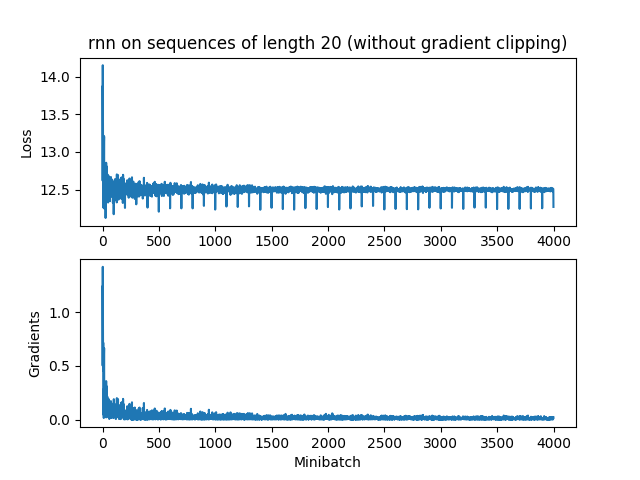
\includegraphics[width=0.6\textwidth]{../code/q3-noclip-rnn.png}
      \caption{Plots of learning dynamics generated for a RNN without gradient clipping.}
      \label{fig1}
    \end{figure}
    \begin{figure}[h]
      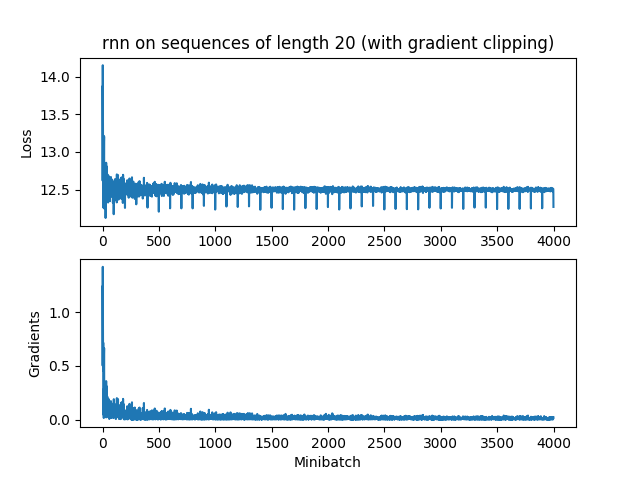
\includegraphics[width=0.6\textwidth]{../code/q3-clip-rnn.png}
      \caption{Plots of learning dynamics generated for a RNN with gradient clipping.}
      \label{fig2}
    \end{figure}
    \begin{figure}[h]
      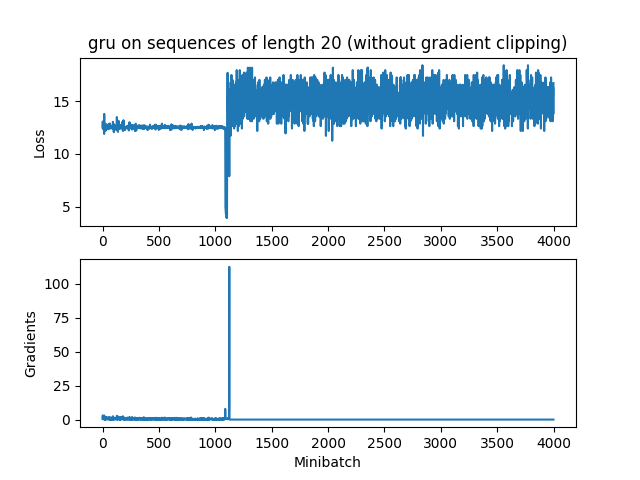
\includegraphics[width=0.6\textwidth]{../code/q3-noclip-gru.png}
      \caption{Plots of learning dynamics generated for a GRU without gradient clipping.}
      \label{fig3}
    \end{figure}
    \begin{figure}[h]
      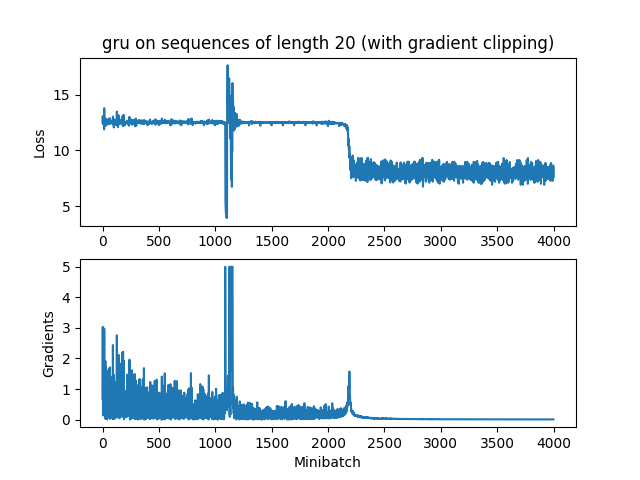
\includegraphics[width=0.6\textwidth]{../code/q3-clip-gru.png}
      \caption{Plots of learning dynamics generated for a GRU with gradient clipping.}
      \label{fig4}
    \end{figure}
  %% Question 3(e)
  \item 
    \begin{enumerate}[itemsep=2ex]
      \item Both RNN models experience vanishing gradients and plateau at a final 
        loss of 12.4978. Gradient clipping does not help with the vanishing gradients problem. 
        Both GRU models experience exploding gradients at around timestep 1100, but in this case 
        gradient clipping helps bring the problem under control. 
      \item The GRU model with gradient clipping performs the best, 
        arriving at a final loss of 8.0668. It is likely because the model is equipped to handle both 
        vanishing gradients (GRU) and exploding gradients (gradient clipping) problems. 
    \end{enumerate}
  %% Question 3(f)
  \item Please see the coding portion of the assignment.
  \end{enumerate}


\end{enumerate}
\end{document}
